% See exam.cls and examdoc.tex for the license information
\documentclass[12pt, answers]{exam}

\usepackage{amssymb}
\usepackage{makeidx}
\usepackage{amsmath}
\usepackage{graphicx}
\usepackage{caption}
\usepackage{tabulary}
\usepackage{color}
\usepackage{multicol}
%\usepackage{multirow}
%\usepackage{enumerate}

\usepackage{array}
\newcolumntype{C}[1]{>{\centering\let\newline\\\arraybackslash\hspace{0pt}}m{#1}}

\addpoints

% In case we're not using hyperref.sty:
\providecommand{\texorpdfstring}[2]{#1}
% The following can be used in \section commands
% without generating pdf warnings:
\newcommand{\bs}{\texorpdfstring{\char`\\}{}}

\makeindex

\newcommand{\indc}[1]{\index{#1@\texttt{\char`\\#1}}}
\newcommand{\indcsub}[2]{\index{#1@\texttt{\char`\\#1}!#2}}
\newcommand{\indcstart}[1]{\index{#1@\texttt{\char`\\#1}|(}}
\newcommand{\indcstop}[1]{\index{#1@\texttt{\char`\\#1}|)}}

\newcommand{\indt}[1]{\index{#1@\texttt{#1}}}
\newcommand{\indtsub}[2]{\index{#1@\texttt{#1}!#2}}
\newcommand{\indtstart}[1]{\index{#1@\texttt{#1}|(}}
\newcommand{\indtstop}[1]{\index{#1@\texttt{#1}|)}}

\extraheadheight{-.4in}

\pagestyle{headandfoot}
%\extraheadheight{.2 in}
\firstpageheader{}{}{}
\runningheader{}{}{}
\firstpagefooter{INF281}{Exercise 02}{Page \thepage\ of \numpages}
\firstpagefootrule
\runningfooter{INF281}{Exercise 02}{Page \thepage\ of \numpages}
\runningfootrule

%---------------------------------------------------------------------

\shadedsolutions
%\noprintanswers
\definecolor{SolutionColor}{rgb}{0.8,0.9,1}

\begin{document}

\section*{INF281 Exercise 02 solutions}

%---------------------------------------------------------------------
\begin{questions}

%%% Question 1
\question \textbf{DP table cell update rules}
  
Dynamic programming (DP) is an algorithm that uses table cells to memorize the sub-solutions of the target solution. DP requires three candidate scores and selects the maximum score among them when updating a cell.

\begin{align*}
H_{i,j}^{(0)} &= H_{i-1,j} - g &(vertical) \\
H_{i,j}^{(1)} &= H_{i,j-1} - g	&(horizontal) \\
H_{i,j}^{(2)} &= H_{i-1,j-1} + R_{a,b} &(diagonal)
\end{align*}

Use the simple scoring scheme below to calcualte $H_{i,j}$ in Table A and B. 

\textbf{Scoring scheme: }\\
\null \quad $R_{ab}$ = 1 for a = b \\ 
\null \quad $R_{ab}$ = 0 for a $\neq$ b \\ 
\null \quad g = 1  

\vspace{0.1 in}

\begin{parts}

%% (a)
\part Table A

\begin{figure}[h]
  \centering
      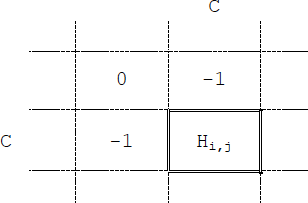
\includegraphics[width=0.325 \textwidth]{fig02/cell_update_1.png}
\end{figure}

\begin{solution}[0.75 in]
1
\end{solution}

%% (b)
\part  Table B

\begin{figure}[!h]
  \centering
      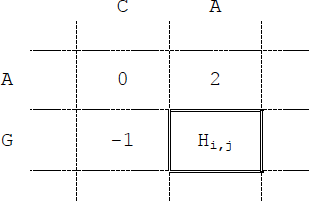
\includegraphics[width=0.325 \textwidth]{fig02/cell_update_2.png}
\end{figure}

\begin{solution}[0.75 in]
1
\end{solution}

\end{parts}

\pagebreak


%%% Question 2
\question \textbf{DP initialization}
  
Initialization is the first step of the DP procedures.

\vspace{0.1 in}

\begin{parts}

%% (a)
\part Initialize the DP table with gap penalty 3.

\begin{figure}[h]
  \centering
      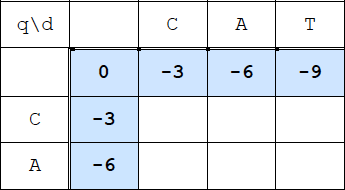
\includegraphics[width=0.35 \textwidth]{fig02/dp_initialization_solution.png}
\end{figure}

\end{parts}

\bigskip 


%%% Question 3
\question \textbf{DP global alignment}
  
The score of optimal global alignment is found in the cell of the bottom-right corner after updating all cells.

\vspace{0.1 in}

\textbf{Scoring scheme: }\\
\null \quad $R_{ab}$ = 1 for a = b \\ 
\null \quad $R_{ab}$ = 0 for a $\neq$ b \\ 
\null \quad g = 1  

\vspace{0.1 in}

\begin{parts}

%% (a)
\part Use the simple scorning scheme and fill the empty cells with appropriate scores.

\begin{figure}[h]
  \centering
      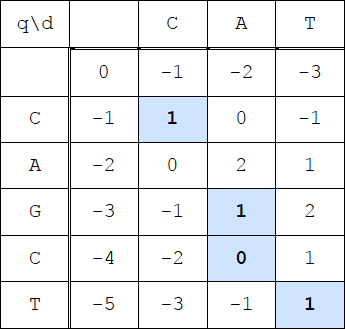
\includegraphics[width=0.35 \textwidth]{fig02/dp_with_simple_score_solution.png}
\end{figure}

%% (b)
\part What is the optimal score of the alignemnt?

\begin{solution}[0.75 in]
1
\end{solution}

\end{parts}

\pagebreak


%%% Question 4
\question \textbf{DP backtrack}
  
Backtracking is a process to find the alignment with the optical score. It requires re-calculations of the three candidate scores.

\vspace{0.1 in}

\textbf{Scoring scheme: }\\
\null \quad $R_{ab}$ = 1 for a = b \\ 
\null \quad $R_{ab}$ = 0 for a $\neq$ b \\ 
\null \quad g = 1  

\vspace{0.1 in}

\begin{parts}

%% (a)
\part Which type of candidate score -- vertical, horizontal, or diagonal -- is used to update the cell with a double border?  Assume that the simple scoring scheme has been used.

\vspace{0.1 in}

\begin{itemize}
\item Table 1
\begin{figure}[h]
  \centering
      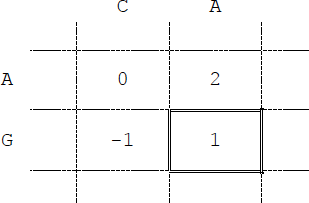
\includegraphics[width=0.25 \textwidth]{fig02/backtrack_recalculate_1.png}
\end{figure}
\begin{solution}[0.25 in]
Vertical
\end{solution}

\item Table 2
\begin{figure}[h]
  \centering
      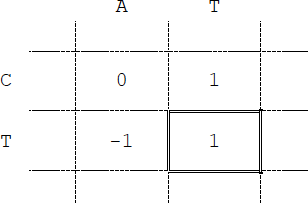
\includegraphics[width=0.25 \textwidth]{fig02/backtrack_recalculate_2.png}
\end{figure}
\begin{solution}[0.25 in]
Diagonal
\end{solution}

\end{itemize}

%% (b)
\part Use backtracking to find the optimal global alignment.
\begin{figure}[h]
  \centering
      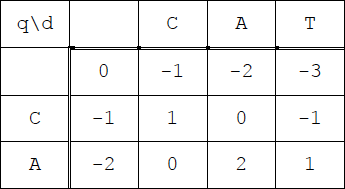
\includegraphics[width=0.3 \textwidth]{fig02/backtrack_simple_table.png}
\end{figure}
\begin{solution}[0.75 in]
\begin{verbatim}
  q: CA-
  d: CAT
\end{verbatim}
\end{solution}

\end{parts}

\bigskip 


%%% Question 5
\question \textbf{DP with score matrix}
  
Use the score matrix below with gap penalty g =1 and answer the following questions.

\begin{figure}[h]
  \centering
      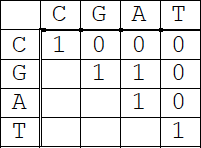
\includegraphics[width=0.2 \textwidth]{fig03/simple_score_matrix.png}
\end{figure}

\begin{parts}

%% (a)
  \part	Calculate the alignment score.

\begin{itemize}
\item Alignment 1
\begin{verbatim}
    q: ATGCT
    d: CA--T \end{verbatim}
    
\begin{solution}[0.35 in]
  1
\end{solution}
  
\item Alignment 2
\begin{verbatim}
    q: CAGCT
    d: C-A-T \end{verbatim}
  
\begin{solution}[0.35 in]
  1
\end{solution}

\end{itemize}

%% (b)
\part Calculate the score of $H_{i,j}$.

\begin{itemize}
\item Table A
\begin{figure}[h]
  \centering
      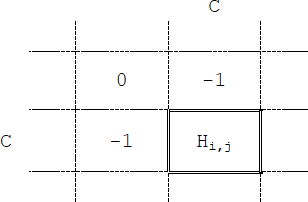
\includegraphics[width=0.25 \textwidth]{fig03/cell_update_score_matrix_1.png}
\end{figure}

\begin{solution}[0.35 in]
1
\end{solution}

\item Table B
\begin{figure}[!h]
  \centering
      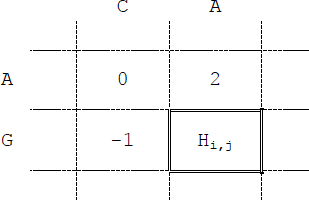
\includegraphics[width=0.25 \textwidth]{fig03/cell_update_score_matrix_2.png}
\end{figure}

\begin{solution}[0.35 in]
1
\end{solution}

\end{itemize}

\pagebreak

%% (c)
\part Fill the empty cells with appropriate scores in the DP table. What is the optimal alignment score?

\begin{figure}[h]
  \centering
      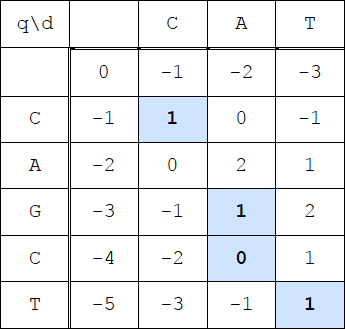
\includegraphics[width=0.35 \textwidth]{fig03/dp_with_score_matrix_solution.png}
\end{figure}

\begin{solution}[0.75 in]
1
\end{solution}

%% (d)
\part There are two different alignments that give the same optimal score in the solution above. Specify both of them.

\begin{solution}[1.75 in]
\begin{verbatim}
  q: CAGCT
  d: CA--T
  
  q: CAGCT
  d: C-A-T
\end{verbatim}
\end{solution}

\end{parts}

\pagebreak


\end{questions}
%---------------------------------------------------------------------
       
\end{document}

